%%%%%%%%%%%%%%%%%%%%%%%%%%%%%%%%%%%%%%%%%%%%%%%%%%%%%%%%%%
\begin{frame}
\frametitle{Spark Components: System-level View}
%%%%%%%%%%%%%%%%%%%%%%%%%%%%%%%%%%%%%%%%%%%%%%%%%%%%%%%%%%
	\begin{figure}[h]
	  \centering
	  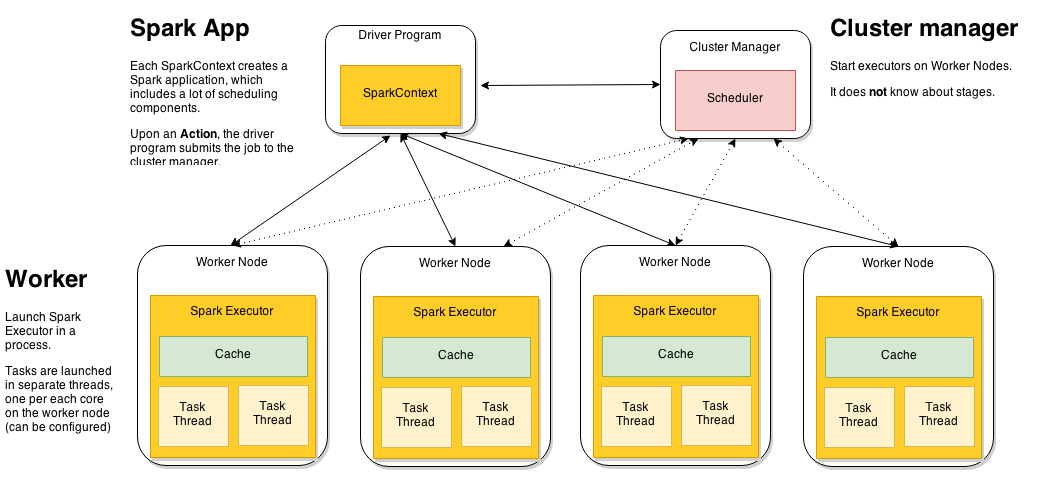
\includegraphics[scale=0.33]{./Figures/spark_system}
	  \label{fig:spark_components}
	\end{figure}
\end{frame}

%%%%%%%%%%%%%%%%%%%%%%%%%%%%%%%%%%%%%%%%%%%%%%%%%%%%%%%%%%
\frame {\frametitle{Spark Components}
%%%%%%%%%%%%%%%%%%%%%%%%%%%%%%%%%%%%%%%%%%%%%%%%%%%%%%%%%%
\begin{figure}[h]
  \centering
  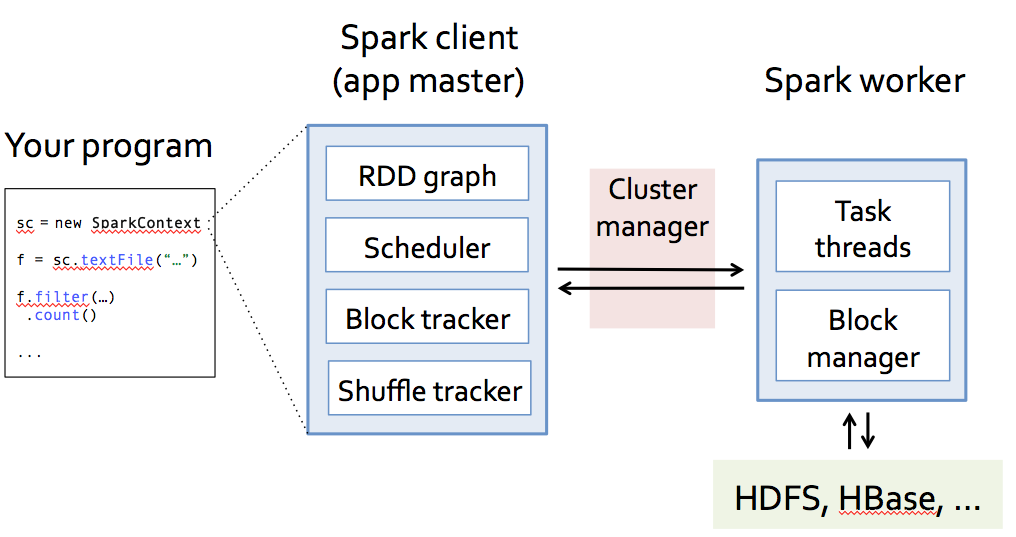
\includegraphics[scale=0.33]{./Figures/spark_components}
  \label{fig:spark_components}
\end{figure}
}

%%%%%%%%%%%%%%%%%%%%%%%%%%%%%%%%%%%%%%%%%%%%%%%%%%%%%%%%%%
\begin{frame}[fragile]
\frametitle{A Very Simple Job Example}
%%%%%%%%%%%%%%%%%%%%%%%%%%%%%%%%%%%%%%%%%%%%%%%%%%%%%%%%%%


\begin{lstlisting}
val sc = new SparkContext("spark://...", "MyJob", home, jars) 

val file = sc.textFile("hdfs://...") // This is an RDD

val errors = file.filter(_.contains("ERROR")) // This is an RDD

errors.cache()

errors.count() // This is an action
\end{lstlisting}

\end{frame}

%%%%%%%%%%%%%%%%%%%%%%%%%%%%%%%%%%%%%%%%%%%%%%%%%%%%%%%%%%
\frame {\frametitle{The RDD graph: dataset vs. partition views}
%%%%%%%%%%%%%%%%%%%%%%%%%%%%%%%%%%%%%%%%%%%%%%%%%%%%%%%%%%
% missing: what is an rdd? difference between RDD and partition?

\begin{columns}[c]
	\column{.5\textwidth}
		
			\begin{figure}[h]
			  \centering
			  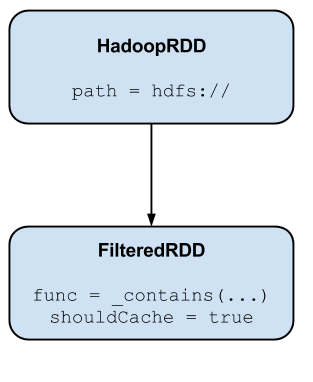
\includegraphics[scale=0.25]{./Figures/spark_rdd}
			  \label{fig:spark_components}
			\end{figure}
	
	\column{.5\textwidth}
		
			\begin{figure}[h]
			  \centering
			  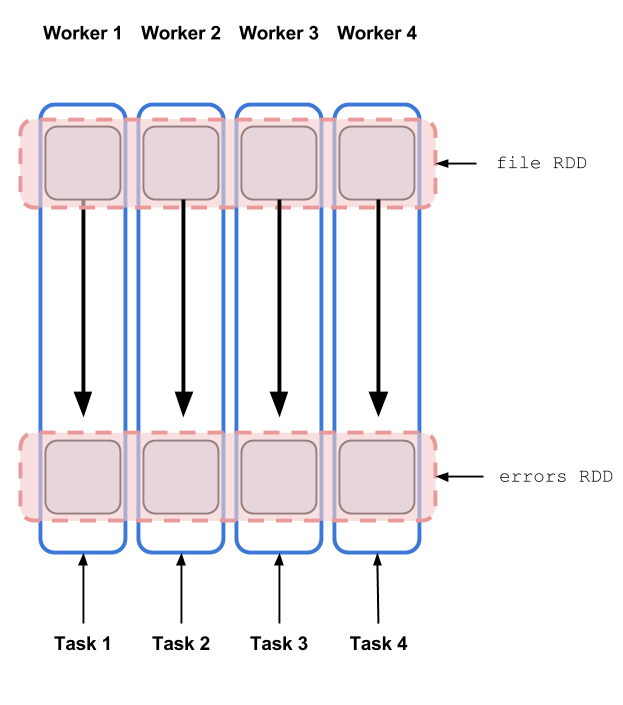
\includegraphics[scale=0.25]{./Figures/spark_partition}
			  \label{fig:spark_components}
			\end{figure}

\end{columns}
}

% %%%%%%%%%%%%%%%%%%%%%%%%%%%%%%%%%%%%%%%%%%%%%%%%%%%%%%%%%%
\frame {\frametitle{Data Locality}
% %%%%%%%%%%%%%%%%%%%%%%%%%%%%%%%%%%%%%%%%%%%%%%%%%%%%%%%%%%
\begin{itemize}
	\item {\bf Data locality principle}
	\begin{itemize}
		\item Same as for Hadoop MapReduce
		\item Avoid network I/O, workers should manage local data
	\end{itemize}

	\vspace{20pt}

	\item {\bf Data locality and caching}
	\begin{itemize}
		\item First run: data not in cache, so use HadoopRDD's locality prefs (from HDFS)
		\item Second run: FilteredRDD is in cache, so use its locations
		\item If something falls out of cache, go back to HDFS
	\end{itemize}
\end{itemize}
}



%%%%%%%%%%%%%%%%%%%%%%%%%%%%%%%%%%%%%%%%%%%%%%%%%%%%%%%%%%
\frame {\frametitle{Lifetime of a Job in Spark}
%%%%%%%%%%%%%%%%%%%%%%%%%%%%%%%%%%%%%%%%%%%%%%%%%%%%%%%%%%

\begin{columns}[t, onlytextwidth]
	\begin{column}[T]{.2\textwidth}
		\begin{center}
			{ \tiny \bf RDD Objects}
		\end{center}
		\begin{figure}[h]
			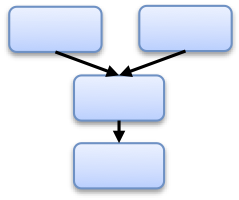
\includegraphics[scale=0.5]{./Figures/RDD_objects}
		\end{figure}

		\begin{colorblock}{blue}{lightblue}{ }
			{\tiny \texttt{
				rdd1.join(rdd2)\\
				\hspace{12pt} .groupBy(...)\\
				\hspace{12pt} .filter(...)\\
				}
			}
		\end{colorblock}

		\vspace{10pt}

		\begin{colorblock}{blue}{lightblue}{ }
			{\tiny \bf Build the operator DAG}
		\end{colorblock}
	\end{column}

	\begin{column}[T]{.2\textwidth}
		\begin{center}
			{ \tiny \bf DAG Scheduler}
		\end{center}			
		\begin{figure}[h]
			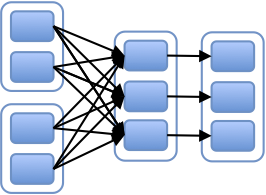
\includegraphics[scale=0.5]{./Figures/DAG_scheduler}
		\end{figure}

		\vspace{10pt}

		\begin{colorblock}{blue}{lightblue}{ }
			{\tiny \bf Split the DAG into \emph{stages} of \emph{tasks}}
		\end{colorblock}

		\vspace{10pt}

		\begin{colorblock}{blue}{lightblue}{ }
			{\tiny \bf Submit each stage and its tasks as ready}
		\end{colorblock}			
	\end{column}

	\begin{column}[T]{.2\textwidth}
		\begin{center}
			{ \tiny \bf Task Scheduler}
		\end{center}			

		\vspace{-20pt}

		\begin{figure}[h]
			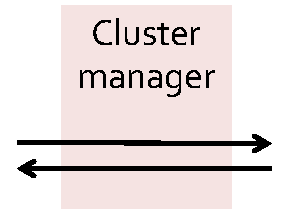
\includegraphics[scale=0.5]{./Figures/Task_scheduler}
		\end{figure}

		\vspace{10pt}

		\begin{colorblock}{blue}{lightblue}{ }
			{\tiny \bf Launch tasks via Master}
		\end{colorblock}

		\vspace{10pt}

		\begin{colorblock}{blue}{lightblue}{ }
			{\tiny \bf Retry failed and straggler tasks}
		\end{colorblock}			
	\end{column}

	\begin{column}[T]{.2\textwidth}
		\begin{center}
			{ \tiny \bf Worker}
		\end{center}			
		\begin{figure}[h]
			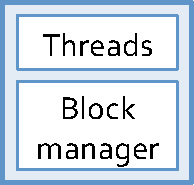
\includegraphics[scale=0.5]{./Figures/Worker}
		\end{figure}
		\vspace{10pt}

		\begin{colorblock}{blue}{lightblue}{ }
			{\tiny \bf Execute tasks}
		\end{colorblock}

		\vspace{10pt}

		\begin{colorblock}{blue}{lightblue}{ }
			{\tiny \bf Store and serve blocks}
		\end{colorblock}			
	\end{column}
\end{columns}
}

